\documentclass[a4paper,oneside]{book}
\usepackage[latin2]{inputenc}
\usepackage[magyar]{babel}
\usepackage{amssymb}
\usepackage{amsmath}
\usepackage[,dvips]{graphicx}
\usepackage{pstricks}
\usepackage{pstricks-add}
\usepackage{pst-3dplot}
\usepackage{pst-plot}
\pagestyle{empty}

\marginparwidth = 0pt
\voffset - 20pt 
\hoffset - 60pt 
\textwidth 450pt
\textheight 700pt
\parindent 0pt

\begin{document}

\textbf{B. 3977.}\\
Kriv�n B�lint\\
Budapest, Berzsenyi D. Gimn., 10. o. t.\\
redhat24@freemail.hu\\

\textbf{Feladat:}\\ Legyenek $x$, $y$, $z$ pozit�v val�s sz�mok, melyekre:
\[x^2+xy+y^2=2\]
\[y^2+yz+z^2=5\]
\[z^2+xz+x^2=3\]

Hat�rozzuk meg $xy+yz+xz$ �rt�k�t!\\
\hrule
\hskip 10pt

\textbf{Megold�s:}\\

�br�zoljuk az els� egyenletet ($x^2+xy+y^2=2$), mint f�ggv�nyt:

\begin{figure}[ht]
\centerline{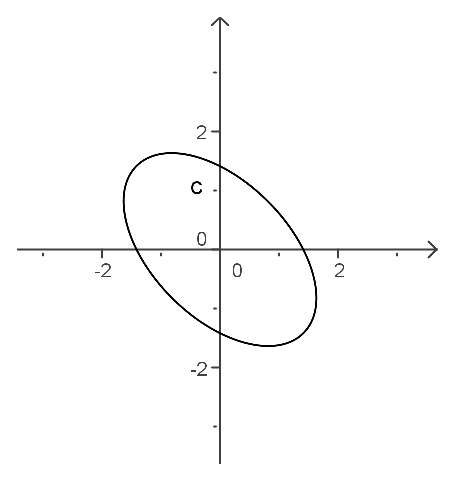
\includegraphics{egyenlet_1.eps}}
\caption{}
\end{figure}

L�thatjuk, hogy ez egy ellipszis. Forgassuk el 45�-al.\\

Pont forgat�sa 45�-al:\\

\[P(x_1; y_1) = P(r\cdot\cos\alpha;r\cdot\sin\alpha)\]
\[P(r\cdot\cos(\alpha+45�);r\cdot\sin(\alpha+45�))\]
\[P(r\cdot\cos\alpha\cos 45�-r\cdot\sin\alpha\sin 45�;r\cdot\sin\alpha\cos 45�+r\cdot\cos\alpha\sin 45�)\]
\[P\Big(r\cdot\frac{\cos\alpha}{\sqrt{2}}-r\cdot\frac{\sin\alpha}{\sqrt{2}};r\cdot\frac{\sin\alpha}{\sqrt{2}}+r\cdot\frac{\cos\alpha}{\sqrt{2}}\Big)\]
\[P\Big(\frac{x_1-y_1}{\sqrt{2}};\frac{y_1+x_1}{\sqrt{2}}\Big)\]

Teh�t, akkor az elforgatott ellipszis�nk k�plete:

\[\Big(\frac{x-y}{\sqrt{2}}\Big)^2+\Big(\frac{x-y}{\sqrt{2}}\Big)\Big(\frac{x+y}{\sqrt{2}}\Big)+\Big(\frac{x+y}{\sqrt{2}}\Big)^2=2\]
Amit egyszer�s�t�nk:
\[\frac{3x^2}{2}+\frac{y^2}{2}=2\]

Hasonl�an megtessz�k ezt a t�bbi egyenlettel/ellipszissel:
\[\frac{3y^2}{2}+\frac{z^2}{2}=5\]
\[\frac{3z^2}{2}+\frac{x^2}{2}=3\]

�sszeadva kapjuk, hogy:
\[2x^2+2y^2+3z^2=10\]
\[x^2+y^2+z^2=5\]
Fontos, hogy az $x$, $y$ �s $z$ m�r a 45�-al elforgatott koordin�tarendszer�nk pontjai!\\

[\dots]\\

Teh�t a $xy+yz+xz$ kifejez�s �rt�ke (sz�mol�g�ppel tal�ltam meg):
\[xy+yz+xz=\pm 2\sqrt{2}\]
\end{document}
